Our method, \METHOD, learns a maximum entropy goal distribution $\pg$ using samples collected from a goal-conditioned policy.
We analyze the algorithm and show that \METHOD maximizes the goal distribution entropy, and present a practical instantiation for unsupervised deep RL.

\subsection{\METHOD Algorithm}\label{sec:method-description}
To learn a uniform distribution over \emph{valid} goal states, we present a method that iteratively increases the entropy of a generative model $\pg$.
In particular, given a generative model $\pgt$ at iteration $t$, we want to train a new generative model, $\pgtt$ that has higher entropy.
While we do not know the set of valid states $\Imgs$, we could sample states \mbox{$\st_n \overset{\text{iid}}{\sim} \pstatet$} using the goal-conditioned policy,
and use the samples to train $\pgtt$.
However, there is no guarantee that this would increase the entropy of $\pgtt$.

\begin{figure}[ht]
    \centering
    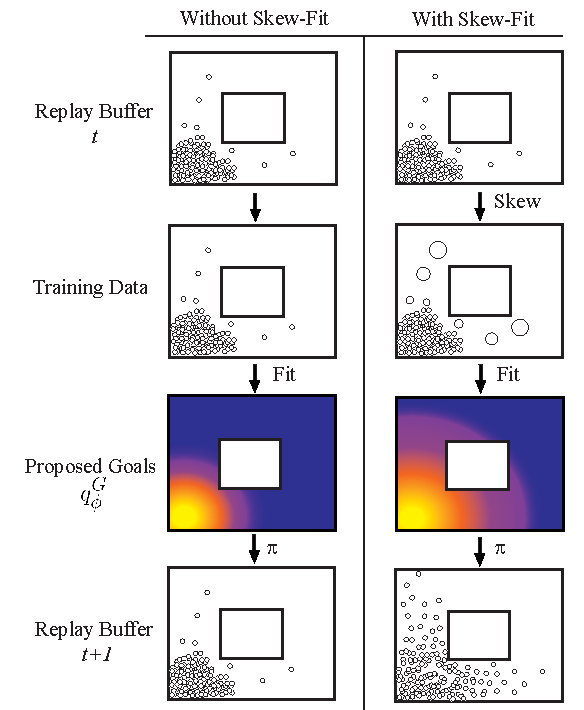
\includegraphics[width=.8\linewidth]{skewfit/figures/skewfitfigure_vertical_q_phi_g.pdf}
    \caption{Our method, \METHOD, samples goals for goal-conditioned RL.
    We sample states from our replay buffer, and give more weight to rare states.
    We then train a generative model $\pg_{t+1}$ with the weighted samples.
    By sampling new states with goals proposed from this new generative model, we obtain a higher entropy state distribution in the next iteration.}
    \label{fig:main-fig}
\end{figure}

The intuition behind our method is simple: rather than fitting a generative model to these samples $\st_n$, we \textit{skew} the samples so that rarely visited states are given more weight.
See \Figref{fig:main-fig} for a visualization of this process.
How should we skew the samples if we want to maximize the entropy of $\pgtt$?
If we had access to the density of each state, $\pet(\St)$, then we could simply weight each state by $1/\pet(\St)$.
We could then perform maximum likelihood estimation (MLE) for the uniform distribution by using the following importance sampling (IS) loss to train $\pgparamtt$:
\begin{align}
\Loss(\pgparam)\nonumber
    &= \E_{\St \sim \U} \left[ \log \pg(\St)\right]
\\\nonumber
    &= \E_{\St \sim \pet}\left[ \frac{\U(\St)}{\pet(\St)} \log \pg(\St)\right]
\\\nonumber
    &\propto \E_{\St \sim \pet}\left[ \frac{1}{\pet(\St)}\log \pg(\St)\right]
\nonumber
\end{align}
where we use the fact that the uniform distribution $\U(\St)$ has constant density for all states in $\Imgs$.
However, computing this density $\pet(\St)$ requires marginalizing out the MDP dynamics, which requires an accurate model of both the dynamics and the goal-conditioned policy.

We avoid needing to model the entire MDP process by approximating $\pet(\St)$ with our previous learned generative model: \mbox{$\pstatet(\St) \approx \pgt(\St)$}.
We therefore weight each state by the following weight function
\begin{align}\label{eq:weight-defn}
    \wt(\SF) \triangleq \pgt(\SF)^\alpha, \quad \alpha < 0.
\end{align}
where $\alpha$ is a hyperparameter that controls how heavily we weight each state.
If our approximation $\pgt$ is exact, we can choose $\alpha = -1$ and recover the exact IS procedure described above.
If $\alpha = 0$, then this skew step has no effect.
By choosing intermediate values of $\alpha$, we trade off the reliability of our estimate $\pgt(\St)$ with the speed at which we want to increase the goal distribution entropy.

\paragraph{Variance Reduction}
As described, this procedure relies on IS, which can have high variance, particularly if $\pgt(\St) \approx 0$.
We therefore choose a class of generative models where the probabilities are prevented from collapsing to zero, as we will describe in \autoref{sec:train-policy} where we provide generative model details.
To further reduce the variance, we train $\pgtt$ with sampling importance resampling (SIR)~\citep{rubin1988using} rather than IS.
Rather than sampling from $\pet$ and weighting the update from each sample by $\wt$, SIR explicitly defines a skewed empirical distribution as
\begin{align}\label{eq:pskew-defn}
    \pskewedt(\st) \triangleq \frac{1}{Z_\alpha} \wt(\st) \delta(\st \in \{\st_n\}_{n=1}^{N})
    \\\nonumber
    Z_\alpha = \sum_{n=1}^N \wt(\st_n),\ \st_n \overset{\text{iid}}{\sim} \pstatet,
\end{align}
where $\delta$ is the indicator function and $Z_\alpha$ is the normalizing coefficient.
We note that computing $Z_\alpha$ adds little computational overhead, since all of the weights already need to be computed.
We then fit the generative model at the next iteration $\pgtt$ to $\pskewedt$ using standard MLE.
We found that using SIR resulted in significantly lower variance than IS.
See \autoref{sec:analysis-variance} for this comparision.

\paragraph{Goal Sampling Alternative}
Because $\pgtt \approx \pskewedt$, at iteration $t+1$, one can sample goals from either $\pgtt$ or $\pskewedt$.
Sampling goals from $\pskewedt$ may be preferred if sampling from the learned generative model $\pgtt$ is computationally or otherwise challenging.
In either case, one still needs to train the generative model $\pgt$ to create $\pskewedt$.
In our experiments, we found that both methods perform well.

\paragraph{Summary}
Overall, \METHOD collects states from the environment and resamples each state in proportion to \autoref{eq:weight-defn} so that low-density states are resampled more often.
\METHOD is shown in \Figref{fig:main-fig} and summarized in Algorithm \ref{alg:method}.
We now discuss conditions under which \METHOD converges to the uniform distribution.

\vspace*{.5cm}
\begin{algorithm}
   	\fcaption{\METHOD}
   	\label{alg:method}
   	\begin{algorithmic}[1]
   	\FOR{Iteration $t=1, 2, ...$}
        \STATE Collect $N$ states $\{\st_n\}_{n=1}^N$ by sampling goals from $\pgt$ (or $\pskewed_{t-1}$) and running goal-conditioned policy.
        \STATE Construct skewed distribution $\pskewedt$ (\Eqref{eq:weight-defn} and \Eqref{eq:pskew-defn}).
        \STATE Fit $\pgtt$ to skewed distribution $\pskewedt$ using MLE.
   	\ENDFOR
   	\end{algorithmic}
\end{algorithm}

\subsection{\METHOD Analysis}\label{sec:analysis}
This section provides conditions under which $\pgt$ converges in the limit to the uniform distribution over the state space $\Imgs$.
We consider the case where $N \rightarrow \infty$, which allows us to study the limit behavior of the goal distribution $\pskewedt$.
Our most general result is stated as follows:
\begin{lemma}\label{lemma:general-convergence}
Let $\Imgs$ be a compact set.
Define the set of distributions $\gQ = \{p : \support(p) \subseteq \Imgs\}$.
Let $\gF: \gQ \mapsto \gQ$ be continuous with respect to the pseudometric \mbox{$\dent(p, q) \triangleq |\gH(p) - \gH(q)|$} and $\gH(\gF(p)) \geq \gH(p)$ with equality if and only if $p$ is the uniform probability distribution on $\Imgs$, denoted as $\U$.
Define the sequence of distributions $P = (p_1, p_2, \dots)$ by starting with any $p_1 \in \gQ$ and recursively defining $p_{t+1} = \gF(p_t)$.
The sequence $P$ converges to $\U$ with respect to $\dent$. In other words, \mbox{$\lim_{t \rightarrow 0} |\gH(p_t) - \gH(\U)| \rightarrow 0$}.
\end{lemma}
\begin{proof}
See Appendix Section \ref{sec:general-proof}.
\end{proof}

We will apply Lemma \ref{lemma:general-convergence} to be the map from $\pskewedt$ to $\pskewedtt$ to show that $\pskewedt$ converges to $\U$.
If we assume that the goal-conditioned policy and generative model learning procedure are well behaved
(i.e., the maps from $\pgt$ to $\pet$ and from $\pskewedt$ to $\pgtt$ are continuous),
then to apply Lemma~\ref{lemma:general-convergence}, we only need to show that \mbox{$\gH(\pskewedt) \geq \gH(\pet)$} with equality if and only if \mbox{$\pet = \U$}.
For the simple case when \mbox{$\pgt = \pet$} identically at each iteration, we prove the convergence of \METHOD true for any value of $\alpha \in [-1, 0)$ in \autoref{sec:simple-case-proof}.
However, in practice, $\pgt$ only approximates $\pet$. To address this more realistic situation, we prove the following result:
\begin{lemma}\label{lemma:pos-cov-negative-grad}
Given two distribution $\pet$ and $\pgt$ where $\pet \ll \pgt$
\footnote{
$p \ll q$ means that $p$ is absolutely continuous with respect to $q$, i.e. $p(\st) = 0 \implies q(\st) = 0$.
}
and
\begin{align}\label{eq:pos-cov}
  \Cov_{\St \sim \pet}\left[\log \pet(\St), \log \pgt(\St)\right] > 0,
\end{align}
define the $\pskewedt$ as in \Eqref{eq:pskew-defn} and take $N \rightarrow \infty$.
Let $\gH_\alpha(\alpha)$ be the entropy of $\pskewedt$ for a fixed $\alpha$.
Then there exists a constant $a < 0$ such that for all $\alpha \in [a, 0)$,
\begin{align*}
    \gH(\pskewedt) =  \gH_\alpha(\alpha) > \gH(\pet).
\end{align*}
\end{lemma}
\begin{proof}
See Appendix Section \ref{sec:covariance-proof}.
\end{proof}
This lemma tells us that our generative model $\pgt$ does not need to exactly fit the sampled states.
Rather, we merely need the log densities of $\pgt$ and $\pet$ to be correlated, which we expect to happen frequently with an accurate goal-conditioned policy, since $\pet$ is the set of states seen when trying to reach goals from $\pgt$.
In this case, if we choose negative values of $\alpha$ that are small enough, then the entropy of $\pskewedt$ will be higher than that of $\pet$.
Empirically, we found that $\alpha$ values as low as $\alpha=-1$ performed well.

In summary, $\pskewedt$ converges to $\U$ under certain assumptions.
Since we train each generative model $\pgtt$ by fitting it to $\pskewedt$ with MLE, $\pgt$ will also converge to $\U$.
